%%% Template originaly created by Karol Kozioł (mail@karol-koziol.net) and modified for ShareLaTeX use

\documentclass[a4paper,11pt]{article}

\usepackage[T1]{fontenc}
\usepackage[utf8]{inputenc}
\usepackage{graphicx}
\usepackage{xcolor}
\usepackage{xfrac}

\renewcommand\familydefault{\sfdefault}
\usepackage{tgheros}
\usepackage[defaultmono]{droidmono}

\usepackage{amsmath,amssymb,amsthm,textcomp}
\usepackage{enumerate}
\usepackage{multicol}
\usepackage{tikz}

\usepackage{geometry}
\geometry{left=25mm,right=25mm,%
bindingoffset=0mm, top=20mm,bottom=20mm}

\graphicspath{ {imgs/} }

\linespread{1.3}

\newcommand{\linia}{\rule{\linewidth}{0.5pt}}

% custom theorems if needed
\newtheoremstyle{mytheor}
    {1ex}{1ex}{\normalfont}{0pt}{\scshape}{.}{1ex}
    {{\thmname{#1 }}{\thmnumber{#2}}{\thmnote{ (#3)}}}

\theoremstyle{mytheor}
\newtheorem{defi}{Definition}

% my own titles
\makeatletter
\renewcommand{\maketitle}{
\begin{center}
\vspace{2ex}
{\huge \textsc{\@title}}
\vspace{1ex}
\\
\linia\\
\@author \hfill \@date
\vspace{4ex}
\end{center}
}
\makeatother
%%%

% custom footers and headers
\usepackage{fancyhdr}
\pagestyle{fancy}
\lhead{}
\chead{}
\rhead{Page \thepage}
\lfoot{N. Mandel}
\cfoot{}
\rfoot{nicolasjohann.mandel@hdr.qut.edu.au}
\renewcommand{\headrulewidth}{0pt}
\renewcommand{\footrulewidth}{0pt}
%

% code listing settings
\usepackage{listings}
\lstset{
    language=Python,
    basicstyle=\ttfamily\small,
    aboveskip={1.0\baselineskip},
    belowskip={1.0\baselineskip},
    columns=fixed,
    extendedchars=true,
    breaklines=true,
    tabsize=4,
    prebreak=\raisebox{0ex}[0ex][0ex]{\ensuremath{\hookleftarrow}},
    frame=lines,
    showtabs=false,
    showspaces=false,
    showstringspaces=false,
    keywordstyle=\color[rgb]{0.627,0.126,0.941},
    commentstyle=\color[rgb]{0.133,0.545,0.133},
    stringstyle=\color[rgb]{01,0,0},
    numbers=left,
    numberstyle=\small,
    stepnumber=1,
    numbersep=10pt,
    captionpos=t,
    escapeinside={\%*}{*)}
}

%%%----------%%%----------%%%----------%%%----------%%%

\begin{document}

\title{Literature Summary and images}

\author{Nicolas Mandel}

\date{05/26/2020}

\maketitle


\section*{Ontologies From Confirmation of Candidature Document}
\subsection{Spatial-Semantic-Information} \label{subsec:LitMapsSpatSem}
\begin{figure*}[th]
\centering
\resizebox{\textwidth}{!}{
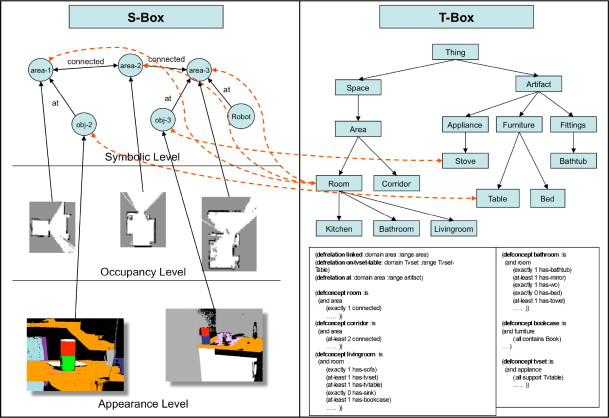
\includegraphics[]{1-0-Galindo-Hierarchy.jpg}}
\caption{A Spatial and Semantic Map as put forward by Galindo et al.~\cite{galindo_robot_2008}}
\label{fig:LitMapsGalindo}
\end{figure*}

\begin{figure*}[t]
\centering
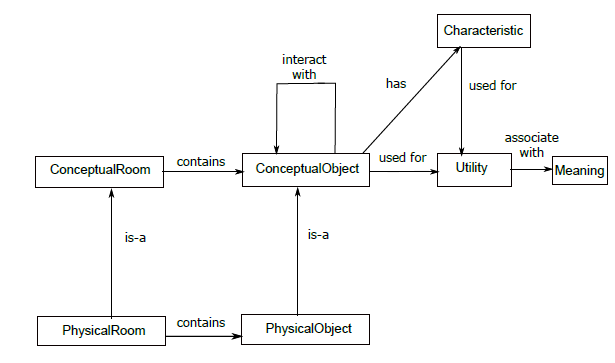
\includegraphics[]{1-2-Crespo-OnotologyForSemNavigation.png}
\caption{An ontology model for semantic navigation suggested by Crespo et al.~\cite{crespo_reasoning_2018}}
\label{fig:LitMapsCrespo}
\end{figure*}
While the approaches to classify, cluster and partition semantic information are numerous~\cite{saffiotti_robots_2011,galindo_robot_2008,crespo_reasoning_2018,tenorth_knowrob-map_2010,cavaliere_empowering_2018,alirezaie_exploiting_2017}, no unanimous conseous on structuring semantic information and maps could be identified, however \textit{ontologies} are generally considered the schema of choice~\cite{kostavelis_semantic_2015}, since they not only model hierarchical relationships in a \textit{taxonomy} similar to WordNet, but also include relationships of influence. These relationships are analogous to gene ontologies, where gene networks are created to display influence in biological settings. The ambiguities surrounding definition of relationships does not hinder the applications of semantic knowledge, which span a wide range and are presented in the following paragraphs.
\begin{figure*}[b]
\centering
\resizebox{\textwidth}{!}{
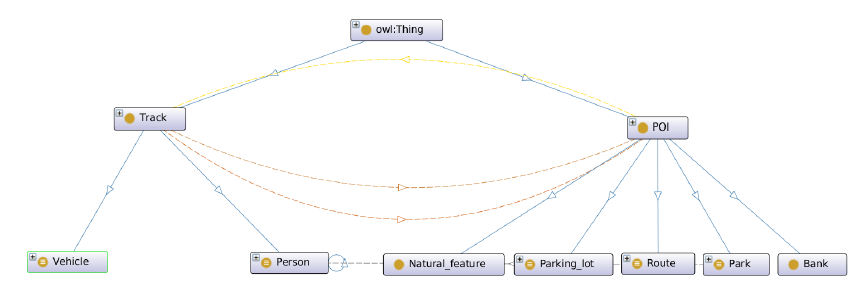
\includegraphics{1-3-Cavaliere-TrackPOIOntology.png}}
\caption{\bf{An ontology to connect trackable objects with places of interest for use with UAVs, defined by Cavaliere et al.~\cite{cavaliere_empowering_2018}}}
\label{fig:LitMapsCavaliere}
\end{figure*} 
Relating to interaction with the environment on a semantic context, Saffiotti~\cite{saffiotti_robots_2011} used semantic context knowledge to infer a goal for a robot to actively restore an order of objects consistent with its internal knowledge. Hemachandra et al.~\cite{hemachandra_learning_2014} developed a method to include language utterances to support identification of semantic regions in indoor environments. Lüddecke and Wörgötter~\cite{luddecke_learning_2017} developed a cost function to segment non-exclusive affordances, but were restricted by limited dataset size.

While all of these approaches are unified by the use of semantic information, the structure of this information is diverse. A few attempts at tackling the relationships are highlighted.
Galindo et al.~\cite{galindo_robot_2008} separate spatial and terminological classifications into two separate boxes, as displayed in~\fig{LitMapsGalindo}. Connections are then made and linked across boxes, as indicated by red dotted lines, which are used to infer potential connections. While reducing planning time with growing terms due to semantic inference, the ontology requires finely tuned in-set definitions.\\

Crespo et al.~\cite{crespo_reasoning_2018} build on the KnowRob-knowledgebase built by Tenorth et al.~\cite{tenorth_knowrob-map_2010} and shown in~\fig{LitMapsCrespo}. Their system relies on a SQL database, while Tenorth published it as a ROS-structure. The requirement to create the database and relations is mentioned by the authors themselves as a significant hurdle, however, this is also necessary for the KnowRob-package.\\
Cavaliere et al.~\cite{cavaliere_empowering_2018} used an ontology representation shown in~\fig{LitMapsCavaliere} to distinguish tracks, such as persons or vehicles, and places of interest and classified events that happened in a spatio-temporal fashion. The definition of candidate events, tracks and places of interest is very task-specific and requires training a proprietary classification and detection mechanism. 
\begin{figure*}[h]
\centering
\resizebox{\textwidth}{!}{
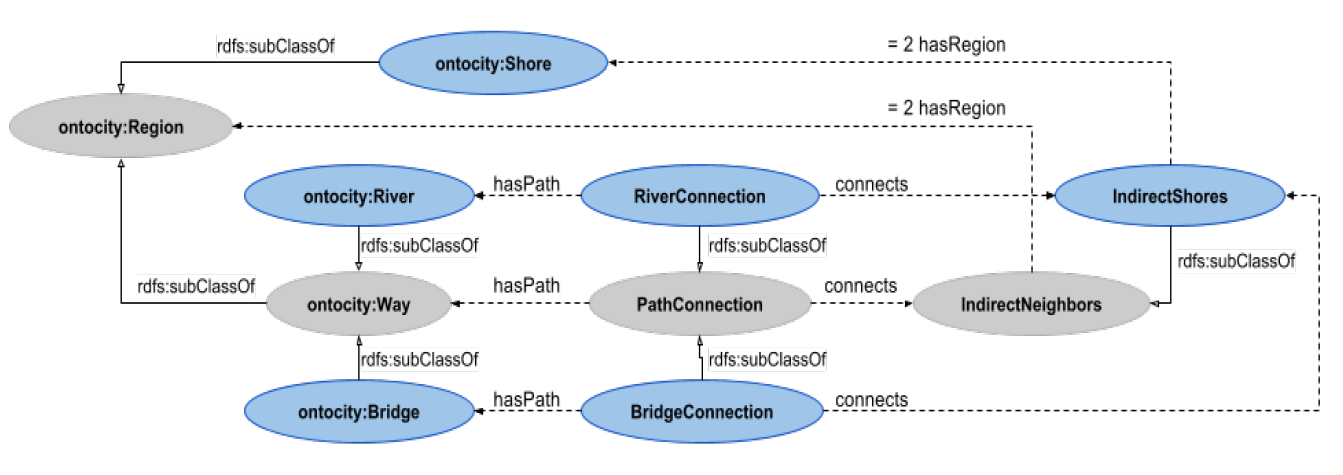
\includegraphics{1-4-Alirezaie-BridgeOntology.png}}
\caption{\bf{A path-connection pattern to define admissible path for UAV RRT-planning, suggested by Alirezaie et al.~\cite{alirezaie_exploiting_2017}}}
\label{fig:LitMapsAlirezaie}
\end{figure*} Alirezaie et al.~\cite{alirezaie_exploiting_2017} created an ontology of areas and connecting pathways, see~\fig{LitMapsAlirezaie}, in an urban setting to create constraints of which regions are considered admissible for waypoints and which are not. This allows them to implement a RRT-path-planner, which is faster at finding safe routes by only allowing certain regions.

While all of these approaches attempt at planning admissible paths or discretising spatial relations and semantic terms, one of the fundamental questions to be answered is where the robot currently is in the map and how certain it is of its location.

\section*{New Stuff}
\begin{itemize}
    \item Toudeshki's approach in image space using an object detector~\cite{toudeshki_robust_2018}
    \item The approach from Tung Dang for Octomaps & 2 classes~\cite{dang_autonomous_2018}
    \item The newest success from chaplot~\cite{chaplot_object_2020,chaplot_learning_2019,chaplot_semantic_2020} referring to Zhang~\cite{zhang_hierarchical_2019} and Wu~\cite{wu_learning_2018}
\end{itemize}

\section*{Stuff from RL and other fields - combining space (image or physical) and a semantic significance}
\begin{itemize}
    \item Niko Suenderhauf's approach for passive mapping~\cite{sunderhauf_meaningful_2017}
    \item Dubey et al's. research on human priors~\cite{dubey_investigating_2018}
    \item The old school approaches from Kuipers~\cite{kuipers_spatial_2000} and~\cite{kuipers_local_2004}
    \item The cognitive linking approaches over development of maps from Eric Chown~\cite{chown_prototypes_1995}
    \item The symbol gorunding problem and its significance from Harnad~\cite{harnad_symbol_1990}
    \item The use of semantic priors in SLAM is mentioned in a seminal paper~\cite{cadena_past_2016}
    \item The use of ''Areas'' or ''Objects'' as new forms of goal for navigtational agents~\cite{anderson_evaluation_2018}
\end{itemize}

Sunderhauf et al.~\cite{sunderhauf_meaningful_2017} state that, while semantic maps may benefit domains such as path planning and manipulation, the investigation of these benefits will in turn show which representations are appropriate and adequate. This underlines the importance of finding ways to include semantic information and posing the question what semantic information representations are available to use with SLAM and semantics.

\section*{UAV Stuff - also from CoC document}
\subsection{UAVs Using Semantics without Motion Planning} \label{subsec:LitUAVPassive}

While multiple efforts of dynamically re-planning UAV paths are ongoing, a few projects focus on the use of semantic features in an aerial context. However, the majority of current research in this area does not include semantic information into active path planning:

Le Saux and Sanfourche~\cite{saux_rapid_2013} used a helicopter to register down-facing images and perform classification on the images during flight. The images were sent to a base station, where a classification algorithm was trained and re-uploaded to classify subsequent images. Even though their learning algorithm was accelerated through an online gradient boosting algorithm, a digital elevation map (DEM) of the environment was required and the classifier had to be trained off-board.

Cavaliere et al.~\cite{cavaliere_towards_2016} classified objects from campus video data and associated places of interest with the collected location information to establish semantic relationships between tracked objects and places. While being able to relate spatial objects within their field of view (FoV), the GPS data is a fundamental component for static object classification and the subject receives no control inputs. More recently, they extended this research to include dynamic events between objects on a higher level of reasoning, while still operating on pre-recorded datasets~\cite{cavaliere_empowering_2018}.

Christie et al.~\cite{christie_semantics_2016} used a semantically-annotated ortophoto created from UAV imagery to navigate an unmanned ground vehicle (UGV) in an urban environment to compare with GPS-based navigation. While gathering semantic information with the UAV, the ground robot generates this information via LIDAR to navigate in a pre-registered environment with five classes: road, grass, ground, building and vegetation. 

In another effort to use semantic information for navigation, Alirezaie et al.~\cite{alirezaie_exploiting_2017} used context information derived from satellite imagery to confine the search space of a rapidly exploring random tree (RRT). While bringing an example of employing semantics in classical navigation algorithms, the algorithm is evaluated on theoretical planning via satellite images, GPS data was needed to obtain information about the location and context knowledge, which is necessary to exploit semantic constraints.

Sheppard and Rahnemoonfar~\cite{sheppard_real-time_2017} classified outdoor top-down UAV imagery into four kinds of scenes, namely buildings, roads, ground and trees. Despite achieving over 90 \% accuracy and a high inference speed on their test dataset, the computations are all conducted offline and the information is not leveraged for path planning.

Kyrkou et al.~\cite{kyrkou_dronet:_2018} benchmarked different self-developed car-detection networks against each other and evaluated them on intersection over union (IoU), frames per second (FPS), precision and sensitivity. The best candidate was deployed on a UAV and tested online on an Odroid and a Raspberry Pi for comparison. Despite running online at more than 10 FPS, they only detected a single class of objects in top-down imagery and did not actively replan trajectories.

Drouilly et al.~\cite{drouilly_semantic_2015} developed a set of metrics for semantic navigation on UAV spherical imagery. The results from a benchmark dataset and simulations showed that the geometrically shortest route does not necessarily correlate with the most semantically salient route. However, their algorithm relied on reference maps and topological submaps and disregarded any object uncertainty. Furthermore, no experiments for active replanning were conducted.

\subsection{UAVs, Semantics and Motion Planning} \label{subsec:LitUAVSemActive}
The literature on using semantic information for motion planning in UAVs is limited. The following papers are deemed the most relevant to our topic.

Showing that modern computational intelligence algorithms based on neural networks are not the only solution, Maravall et al.~\cite{maravall_navigation_2017} used the concept of image entropy stemming from the 1960s to guide their UAV towards semantically salient, pre-registered landmarks by adjusting the steering angle towards areas of high entropy. While showing the effectiveness of an algorithm including obstacle avoidance (by circumventing) without banking on modern computational intelligence, the navigation is relying on a known landmark sequence with heading information.

Maturana et al.~\cite{maturana_looking_2017} developed a NN algorithm to detect cars from an oblique UAV imagery viewpoint and recursively used the information for an online motion-planner to inspect them by moving closer. While identifying a problem with the viewpoint discrepancy between oblique imagery and standardised datasets and solving it by sourcing videos from the World Wide Web, they only scout for a single class and are reliant on elevation information to identify the cars. This paper highlights the issue and limitations of small object detection and dataset influence, which are relevant to general object detection as discussed in~\cite{liu_deep_2019} and highly to UAVs.

Dang et al.~\cite{dang_autonomous_2018} employed a NN online to detected two classes (a mannequin and a bike) while using a RRT path-planner to balance between exploration and information gain. The project combined semantic navigation with a state-of-the-art path-planning algorithm. However, their method was only evaluated in an artificially created environment and relied on a mapping of the space into voxels, which can be computationally expensive with an expanding map size.

Most recently, Toudeshki et al.~\cite{toudeshki_robust_2018} used a state-of-the-art object detection algorithm to track a trajectory in image space for the UAV to autonomously align with. They employed a lane-filtering controller and a self-developed anticipatory control to adjust the course of the UAV to reach a goal. While their use of semantically salient objects as navigation cues is closest to our research, computations are still run off-board, navigation relies on a predefined trajectory and the environment is artificially created to suit the object detector, thus limiting the potential application to new fields.

\bibliographystyle{IEEEtran}
\bibliography{references}
\end{document}